% inspired from http://tex.stackexchange.com/questions/56611/make-a-vigen%C3%A8re-rectangular-in-latex
\documentclass{article}

\usepackage{tikz}
\usetikzlibrary{positioning}
\usepackage{amsmath}

\begin{document}

% Exemple d'utilisation du chiffre de Vigenère

% Chiffrement

% Clé de chiffrement


\begin{tikzpicture}
   \node [minimum size = 0.5cm, inner sep = 0pt] (first) {P};
   \node [minimum size = 0.5cm, inner sep = 0pt, right = 0cm of first] (second) {R};
   \node [minimum size = 0.5cm, inner sep = 0pt, right = 0cm of second] (third) {O};
   \node [minimum size = 0.5cm, inner sep = 0pt, right = 0cm of third] (fourth) {G};
   \node [minimum size = 0.5cm, inner sep = 0pt, right = 0cm of fourth] (fifth) {R};
   \node [minimum size = 0.5cm, inner sep = 0pt, right = 0cm of fifth] (sixth) {A};
   \node [minimum size = 0.5cm, inner sep = 0pt, right = 0cm of sixth] (seventh) {M};
   \node [minimum size = 0.5cm, inner sep = 0pt, right = 0cm of seventh] (eighth) {M};
   \node [minimum size = 0.5cm, inner sep = 0pt, right = 0cm of eighth] (ninth) {A};
   \node [minimum size = 0.5cm, inner sep = 0pt, right = 0cm of ninth] (tenth) {T};
   \node [minimum size = 0.5cm, inner sep = 0pt, right = 0cm of tenth] (eleventh) {I};
   \node [minimum size = 0.5cm, inner sep = 0pt, right = 0cm of eleventh] (twelfth) {O};
   \node [minimum size = 0.5cm, inner sep = 0pt, right = 0cm of twelfth] (thirteenth) {N};
\end{tikzpicture}


\begin{tikzpicture}
   \node [minimum size = 0.5cm, inner sep = 0pt] (first) {L};
   \node [minimum size = 0.5cm, inner sep = 0pt, right = 0cm of first] (second) {I};
   \node [minimum size = 0.5cm, inner sep = 0pt, right = 0cm of second] (third) {N};
   \node [minimum size = 0.5cm, inner sep = 0pt, right = 0cm of third] (fourth) {U};
   \node [minimum size = 0.5cm, inner sep = 0pt, right = 0cm of fourth] (fifth) {X};
   \node [minimum size = 0.5cm, inner sep = 0pt, right = 0cm of fifth] (sixth) {L};
   \node [minimum size = 0.5cm, inner sep = 0pt, right = 0cm of sixth] (seventh) {I};
   \node [minimum size = 0.5cm, inner sep = 0pt, right = 0cm of seventh] (eighth) {N};
   \node [minimum size = 0.5cm, inner sep = 0pt, right = 0cm of eighth] (ninth) {U};
   \node [minimum size = 0.5cm, inner sep = 0pt, right = 0cm of ninth] (tenth) {X};
   \node [minimum size = 0.5cm, inner sep = 0pt, right = 0cm of tenth] (eleventh) {L};
   \node [minimum size = 0.5cm, inner sep = 0pt, right = 0cm of eleventh] (twelfth) {I};
   \node [minimum size = 0.5cm, inner sep = 0pt, right = 0cm of twelfth] (thirteenth) {N};
\end{tikzpicture}

\vspace{1cm}

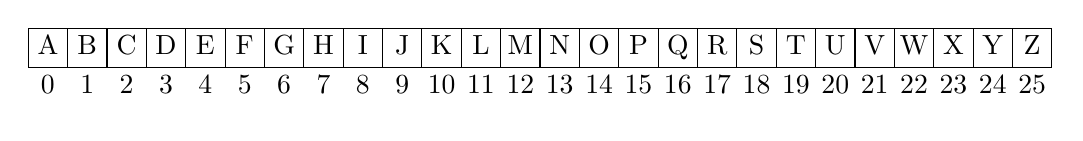
\begin{tikzpicture}
   \foreach \i in {0,...,25} {
      \foreach \j in {0,...,0} {
         \edef\k{\ifnum\numexpr\i+\j\relax>25
            \the\numexpr\i+\j-26\relax
            \else
            \the\numexpr\i+\j\relax
         \fi}
         \node[draw,minimum size=0.5cm,inner sep=0pt]
         at (\i*0.5,-\j*0.5) {\strut\symbol{\numexpr`A+\k\relax}};
      }
      \node at (\i*0.5,-0.5)   {\strut\i};
   }
\end{tikzpicture}

% tour 1

\vspace{1cm}

\begin{tikzpicture}
   \node [minimum size = 0.5cm, inner sep = 0pt] (first) {P $(15e)$};
   \node [minimum size = 0.5cm, inner sep = 0pt, below = 0cm of first] (second) {+};
   \node [minimum size = 0.5cm, inner sep = 0pt, below = 0cm of second] (third) {L $(11e)$};
   \node [minimum size = 0.5cm, inner sep = 0pt, below = 0cm of third] (fourth) {=};
   \node [minimum size = 0.5cm, inner sep = 0pt, below = 0cm of fourth] (fifth) {A $((15 + 11) \mod{26} = 0e)$};
   \node [minimum size = 0.5cm, inner sep = 0pt, above right = 1cm and 2cm of fifth] (sixth) {A};
\end{tikzpicture}

% tour 2

\vspace{1cm}

\begin{tikzpicture}
   \node [minimum size = 0.5cm, inner sep = 0pt] (first) {R $(17e)$};
   \node [minimum size = 0.5cm, inner sep = 0pt, below = 0cm of first] (second) {+};
   \node [minimum size = 0.5cm, inner sep = 0pt, below = 0cm of second] (third) {I $(8e)$};
   \node [minimum size = 0.5cm, inner sep = 0pt, below = 0cm of third] (fourth) {=};
   \node [minimum size = 0.5cm, inner sep = 0pt, below = 0cm of fourth] (fifth) {Z $((17 + 8) \mod{26} = 25e)$};
   \node [minimum size = 0.5cm, inner sep = 0pt, above right = 1cm and 2cm of fifth] (sixth) {A};
   \node [minimum size = 0.5cm, inner sep = 0pt, right = 0cm of sixth] (seventh) {Z};
\end{tikzpicture}

% tour 3

\vspace{1cm}

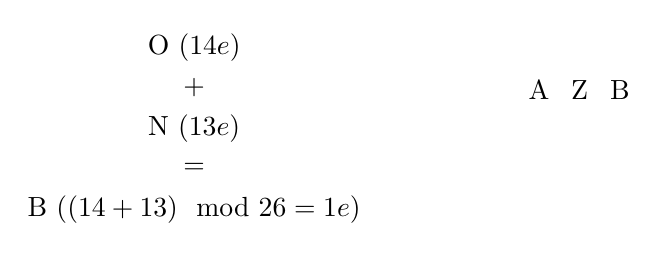
\begin{tikzpicture}
   \node [minimum size = 0.5cm, inner sep = 0pt] (first) {O $(14e)$};
   \node [minimum size = 0.5cm, inner sep = 0pt, below = 0cm of first] (second) {+};
   \node [minimum size = 0.5cm, inner sep = 0pt, below = 0cm of second] (third) {N $(13e)$};
   \node [minimum size = 0.5cm, inner sep = 0pt, below = 0cm of third] (fourth) {=};
   \node [minimum size = 0.5cm, inner sep = 0pt, below = 0cm of fourth] (fifth) {B $((14 + 13) \mod{26} = 1e)$};
   \node [minimum size = 0.5cm, inner sep = 0pt, above right = 1cm and 2cm of fifth] (sixth) {A};
   \node [minimum size = 0.5cm, inner sep = 0pt, right = 0cm of sixth] (seventh) {Z};
   \node [minimum size = 0.5cm, inner sep = 0pt, right = 0cm of seventh] (eighth) {B};
\end{tikzpicture}

\vspace{0.5cm}

\begin{tikzpicture}
   \node [anchor = center] (first) {...};
\end{tikzpicture}

\vspace{0.5cm}

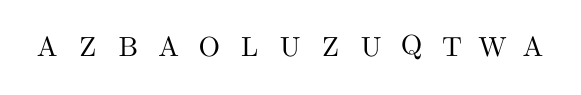
\begin{tikzpicture}
   \node [minimum size = 0.5cm, inner sep = 0pt] (first) {A};
   \node [minimum size = 0.5cm, inner sep = 0pt, right = 0cm of first] (second) {Z};
   \node [minimum size = 0.5cm, inner sep = 0pt, right = 0cm of second] (third) {B};
   \node [minimum size = 0.5cm, inner sep = 0pt, right = 0cm of third] (fourth) {A};
   \node [minimum size = 0.5cm, inner sep = 0pt, right = 0cm of fourth] (fifth) {O};
   \node [minimum size = 0.5cm, inner sep = 0pt, right = 0cm of fifth] (sixth) {L};
   \node [minimum size = 0.5cm, inner sep = 0pt, right = 0cm of sixth] (seventh) {U};
   \node [minimum size = 0.5cm, inner sep = 0pt, right = 0cm of seventh] (eighth) {Z};
   \node [minimum size = 0.5cm, inner sep = 0pt, right = 0cm of eighth] (ninth) {U};
   \node [minimum size = 0.5cm, inner sep = 0pt, right = 0cm of ninth] (tenth) {Q};
   \node [minimum size = 0.5cm, inner sep = 0pt, right = 0cm of tenth] (eleventh) {T};
   \node [minimum size = 0.5cm, inner sep = 0pt, right = 0cm of eleventh] (twelfth) {W};
   \node [minimum size = 0.5cm, inner sep = 0pt, right = 0cm of twelfth] (thirteenth) {A};
\end{tikzpicture}

% Déchiffrement

\newpage

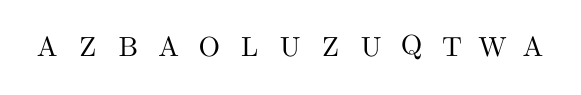
\begin{tikzpicture}
   \node [minimum size = 0.5cm, inner sep = 0pt] (first) {A};
   \node [minimum size = 0.5cm, inner sep = 0pt, right = 0cm of first] (second) {Z};
   \node [minimum size = 0.5cm, inner sep = 0pt, right = 0cm of second] (third) {B};
   \node [minimum size = 0.5cm, inner sep = 0pt, right = 0cm of third] (fourth) {A};
   \node [minimum size = 0.5cm, inner sep = 0pt, right = 0cm of fourth] (fifth) {O};
   \node [minimum size = 0.5cm, inner sep = 0pt, right = 0cm of fifth] (sixth) {L};
   \node [minimum size = 0.5cm, inner sep = 0pt, right = 0cm of sixth] (seventh) {U};
   \node [minimum size = 0.5cm, inner sep = 0pt, right = 0cm of seventh] (eighth) {Z};
   \node [minimum size = 0.5cm, inner sep = 0pt, right = 0cm of eighth] (ninth) {U};
   \node [minimum size = 0.5cm, inner sep = 0pt, right = 0cm of ninth] (tenth) {Q};
   \node [minimum size = 0.5cm, inner sep = 0pt, right = 0cm of tenth] (eleventh) {T};
   \node [minimum size = 0.5cm, inner sep = 0pt, right = 0cm of eleventh] (twelfth) {W};
   \node [minimum size = 0.5cm, inner sep = 0pt, right = 0cm of twelfth] (thirteenth) {A};
\end{tikzpicture}


\begin{tikzpicture}
   \node [minimum size = 0.5cm, inner sep = 0pt] (first) {L};
   \node [minimum size = 0.5cm, inner sep = 0pt, right = 0cm of first] (second) {I};
   \node [minimum size = 0.5cm, inner sep = 0pt, right = 0cm of second] (third) {N};
   \node [minimum size = 0.5cm, inner sep = 0pt, right = 0cm of third] (fourth) {U};
   \node [minimum size = 0.5cm, inner sep = 0pt, right = 0cm of fourth] (fifth) {X};
   \node [minimum size = 0.5cm, inner sep = 0pt, right = 0cm of fifth] (sixth) {L};
   \node [minimum size = 0.5cm, inner sep = 0pt, right = 0cm of sixth] (seventh) {I};
   \node [minimum size = 0.5cm, inner sep = 0pt, right = 0cm of seventh] (eighth) {N};
   \node [minimum size = 0.5cm, inner sep = 0pt, right = 0cm of eighth] (ninth) {U};
   \node [minimum size = 0.5cm, inner sep = 0pt, right = 0cm of ninth] (tenth) {X};
   \node [minimum size = 0.5cm, inner sep = 0pt, right = 0cm of tenth] (eleventh) {L};
   \node [minimum size = 0.5cm, inner sep = 0pt, right = 0cm of eleventh] (twelfth) {I};
   \node [minimum size = 0.5cm, inner sep = 0pt, right = 0cm of twelfth] (thirteenth) {N};
\end{tikzpicture}

\vspace{1cm}

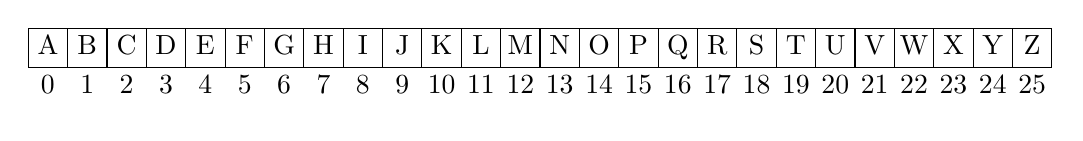
\begin{tikzpicture}
   \foreach \i in {0,...,25} {
      \foreach \j in {0,...,0} {
         \edef\k{\ifnum\numexpr\i+\j\relax>25
            \the\numexpr\i+\j-26\relax
            \else
            \the\numexpr\i+\j\relax
         \fi}
         \node[draw,minimum size=0.5cm,inner sep=0pt]
         at (\i*0.5,-\j*0.5) {\strut\symbol{\numexpr`A+\k\relax}};
      }
      \node at (\i*0.5,-0.5)   {\strut\i};
   }
\end{tikzpicture}

% tour 1

\vspace{1cm}

\begin{tikzpicture}
   \node [minimum size = 0.5cm, inner sep = 0pt] (first) {A $(0e)$};
   \node [minimum size = 0.5cm, inner sep = 0pt, below = 0cm of first] (second) {-};
   \node [minimum size = 0.5cm, inner sep = 0pt, below = 0cm of second] (third) {L $(11e)$};
   \node [minimum size = 0.5cm, inner sep = 0pt, below = 0cm of third] (fourth) {=};
   \node [minimum size = 0.5cm, inner sep = 0pt, below = 0cm of fourth] (fifth) {P $((0 - 11) \mod{26} = 15e)$};
   \node [minimum size = 0.5cm, inner sep = 0pt, above right = 1cm and 2cm of fifth] (sixth) {P};
\end{tikzpicture}

% tour 2

\vspace{1cm}

\begin{tikzpicture}
   \node [minimum size = 0.5cm, inner sep = 0pt] (first) {Z $(25e)$};
   \node [minimum size = 0.5cm, inner sep = 0pt, below = 0cm of first] (second) {-};
   \node [minimum size = 0.5cm, inner sep = 0pt, below = 0cm of second] (third) {I $(8e)$};
   \node [minimum size = 0.5cm, inner sep = 0pt, below = 0cm of third] (fourth) {=};
   \node [minimum size = 0.5cm, inner sep = 0pt, below = 0cm of fourth] (fifth) {R $((25 - 8) \mod{26} = 17e)$};
   \node [minimum size = 0.5cm, inner sep = 0pt, above right = 1cm and 2cm of fifth] (sixth) {P};
   \node [minimum size = 0.5cm, inner sep = 0pt, right = 0cm of sixth] (seventh) {R};
\end{tikzpicture}

% tour 3

\vspace{1cm}

\begin{tikzpicture}
   \node [minimum size = 0.5cm, inner sep = 0pt] (first) {B $(1e)$};
   \node [minimum size = 0.5cm, inner sep = 0pt, below = 0cm of first] (second) {-};
   \node [minimum size = 0.5cm, inner sep = 0pt, below = 0cm of second] (third) {N $(13e)$};
   \node [minimum size = 0.5cm, inner sep = 0pt, below = 0cm of third] (fourth) {=};
   \node [minimum size = 0.5cm, inner sep = 0pt, below = 0cm of fourth] (fifth) {O $((1 - 13) \mod{26} = 14e)$};
   \node [minimum size = 0.5cm, inner sep = 0pt, above right = 1cm and 2cm of fifth] (sixth) {P};
   \node [minimum size = 0.5cm, inner sep = 0pt, right = 0cm of sixth] (seventh) {R};
   \node [minimum size = 0.5cm, inner sep = 0pt, right = 0cm of seventh] (eighth) {O};
\end{tikzpicture}

\vspace{0.5cm}

\begin{tikzpicture}
   \node [anchor = center] (first) {...};
\end{tikzpicture}

\vspace{0.5cm}


\begin{tikzpicture}
   \node [minimum size = 0.5cm, inner sep = 0pt] (first) {P};
   \node [minimum size = 0.5cm, inner sep = 0pt, right = 0cm of first] (second) {R};
   \node [minimum size = 0.5cm, inner sep = 0pt, right = 0cm of second] (third) {O};
   \node [minimum size = 0.5cm, inner sep = 0pt, right = 0cm of third] (fourth) {G};
   \node [minimum size = 0.5cm, inner sep = 0pt, right = 0cm of fourth] (fifth) {R};
   \node [minimum size = 0.5cm, inner sep = 0pt, right = 0cm of fifth] (sixth) {A};
   \node [minimum size = 0.5cm, inner sep = 0pt, right = 0cm of sixth] (seventh) {M};
   \node [minimum size = 0.5cm, inner sep = 0pt, right = 0cm of seventh] (eighth) {M};
   \node [minimum size = 0.5cm, inner sep = 0pt, right = 0cm of eighth] (ninth) {A};
   \node [minimum size = 0.5cm, inner sep = 0pt, right = 0cm of ninth] (tenth) {T};
   \node [minimum size = 0.5cm, inner sep = 0pt, right = 0cm of tenth] (eleventh) {I};
   \node [minimum size = 0.5cm, inner sep = 0pt, right = 0cm of eleventh] (twelfth) {O};
   \node [minimum size = 0.5cm, inner sep = 0pt, right = 0cm of twelfth] (thirteenth) {N};
\end{tikzpicture}

% Table de Vigenère

\newpage

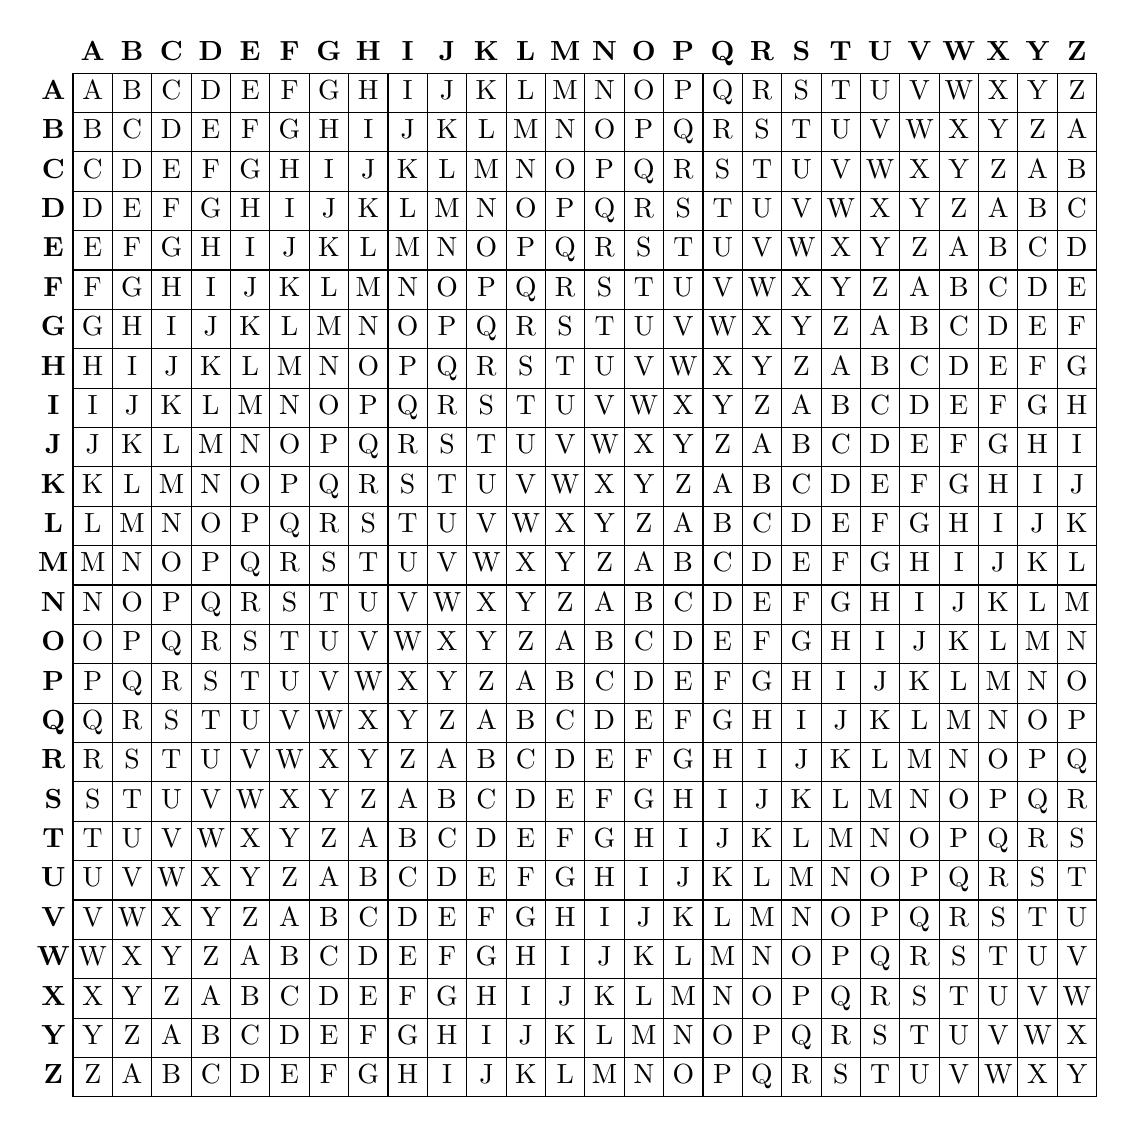
\begin{tikzpicture}
   \foreach \i in {0,...,25} {
      \foreach \j in {0,...,25} {
         \edef\k{\ifnum\numexpr\i+\j\relax>25
            \the\numexpr\i+\j-26\relax
            \else
            \the\numexpr\i+\j\relax
         \fi}
         \node[draw,minimum size=0.5cm,inner sep=0pt]
         at (\i*0.5,-\j*0.5) {\strut\symbol{\numexpr`A+\k\relax}};
      }
      \node [font = \bf] at (-0.5,-\i*0.5) {\strut\symbol{\numexpr`A+\i}};
      \node [font = \bf] at (\i*0.5,0.5)   {\strut\symbol{\numexpr`A+\i}};
   }
\end{tikzpicture}

% Cassage

\newpage

% Ligne 1
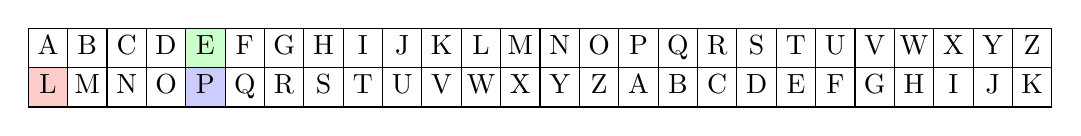
\begin{tikzpicture}
   \foreach \i in {0,...,3} {
      \node[draw, minimum size = 0.5cm, inner sep = 0pt]
      at (\i*0.5,0) {\strut\symbol{\numexpr`A+\i\relax}};
   }
   \foreach \i in {4,...,4} {
      \node[draw, minimum size = 0.5cm, inner sep = 0pt, fill = green!20]
      at (\i*0.5,0) {\strut\symbol{\numexpr`A+\i\relax}};
   }
   \foreach \i in {5,...,25} {
      \node[draw, minimum size = 0.5cm, inner sep = 0pt]
      at (\i*0.5,0) {\strut\symbol{\numexpr`A+\i\relax}};
   }

   \foreach \i in {0,...,0} {
      \foreach \j in {11,...,11} {
         \edef\k{\ifnum\numexpr\i+\j\relax>25
            \the\numexpr\i+\j-26\relax
            \else
            \the\numexpr\i+\j\relax
         \fi}
         \node[draw, minimum size = 0.5cm, inner sep = 0pt, fill = red!20]
         at (\i*0.5,-0.5) {\strut\symbol{\numexpr`A+\k\relax}};
      }
   }
   \foreach \i in {1,...,3} {
      \foreach \j in {11,...,11} {
         \edef\k{\ifnum\numexpr\i+\j\relax>25
            \the\numexpr\i+\j-26\relax
            \else
            \the\numexpr\i+\j\relax
         \fi}
         \node[draw, minimum size = 0.5cm, inner sep = 0pt]
         at (\i*0.5,-0.5) {\strut\symbol{\numexpr`A+\k\relax}};
      }
   }
   \foreach \i in {4,...,4} {
      \foreach \j in {11,...,11} {
         \edef\k{\ifnum\numexpr\i+\j\relax>25
            \the\numexpr\i+\j-26\relax
            \else
            \the\numexpr\i+\j\relax
         \fi}
         \node[draw, minimum size = 0.5cm, inner sep = 0pt, fill = blue!20]
         at (\i*0.5,-0.5) {\strut\symbol{\numexpr`A+\k\relax}};
      }
   }
   \foreach \i in {5,...,25} {
      \foreach \j in {11,...,11} {
         \edef\k{\ifnum\numexpr\i+\j\relax>25
            \the\numexpr\i+\j-26\relax
            \else
            \the\numexpr\i+\j\relax
         \fi}
         \node[draw, minimum size = 0.5cm, inner sep = 0pt]
         at (\i*0.5,-0.5) {\strut\symbol{\numexpr`A+\k\relax}};
      }
   }
\end{tikzpicture}

\vspace{0.5cm}

% Ligne 2
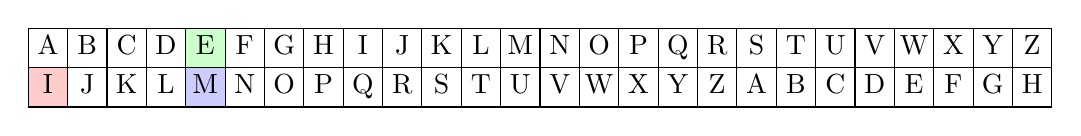
\begin{tikzpicture}
   \foreach \i in {0,...,3} {
      \node[draw, minimum size = 0.5cm, inner sep = 0pt]
      at (\i*0.5,0) {\strut\symbol{\numexpr`A+\i\relax}};
   }
   \foreach \i in {4,...,4} {
      \node[draw, minimum size = 0.5cm, inner sep = 0pt, fill = green!20]
      at (\i*0.5,0) {\strut\symbol{\numexpr`A+\i\relax}};
   }
   \foreach \i in {5,...,25} {
      \node[draw, minimum size = 0.5cm, inner sep = 0pt]
      at (\i*0.5,0) {\strut\symbol{\numexpr`A+\i\relax}};
   }

   \foreach \i in {0,...,0} {
      \foreach \j in {8,...,8} {
         \edef\k{\ifnum\numexpr\i+\j\relax>25
            \the\numexpr\i+\j-26\relax
            \else
            \the\numexpr\i+\j\relax
         \fi}
         \node[draw, minimum size = 0.5cm, inner sep = 0pt, fill = red!20]
         at (\i*0.5,-0.5) {\strut\symbol{\numexpr`A+\k\relax}};
      }
   }
   \foreach \i in {1,...,3} {
      \foreach \j in {8,...,8} {
         \edef\k{\ifnum\numexpr\i+\j\relax>25
            \the\numexpr\i+\j-26\relax
            \else
            \the\numexpr\i+\j\relax
         \fi}
         \node[draw, minimum size = 0.5cm, inner sep = 0pt]
         at (\i*0.5,-0.5) {\strut\symbol{\numexpr`A+\k\relax}};
      }
   }
   \foreach \i in {4,...,4} {
      \foreach \j in {8,...,8} {
         \edef\k{\ifnum\numexpr\i+\j\relax>25
            \the\numexpr\i+\j-26\relax
            \else
            \the\numexpr\i+\j\relax
         \fi}
         \node[draw, minimum size = 0.5cm, inner sep = 0pt, fill = blue!20]
         at (\i*0.5,-0.5) {\strut\symbol{\numexpr`A+\k\relax}};
      }
   }
   \foreach \i in {5,...,25} {
      \foreach \j in {8,...,8} {
         \edef\k{\ifnum\numexpr\i+\j\relax>25
            \the\numexpr\i+\j-26\relax
            \else
            \the\numexpr\i+\j\relax
         \fi}
         \node[draw, minimum size = 0.5cm, inner sep = 0pt]
         at (\i*0.5,-0.5) {\strut\symbol{\numexpr`A+\k\relax}};
      }
   }
\end{tikzpicture}

\vspace{0.5cm}

% Ligne 3
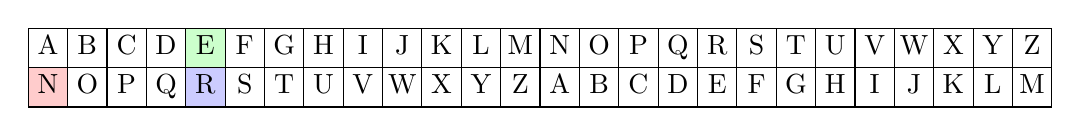
\begin{tikzpicture}
   \foreach \i in {0,...,3} {
      \node[draw, minimum size = 0.5cm, inner sep = 0pt]
      at (\i*0.5,0) {\strut\symbol{\numexpr`A+\i\relax}};
   }
   \foreach \i in {4,...,4} {
      \node[draw, minimum size = 0.5cm, inner sep = 0pt, fill = green!20]
      at (\i*0.5,0) {\strut\symbol{\numexpr`A+\i\relax}};
   }
   \foreach \i in {5,...,25} {
      \node[draw, minimum size = 0.5cm, inner sep = 0pt]
      at (\i*0.5,0) {\strut\symbol{\numexpr`A+\i\relax}};
   }

   \foreach \i in {0,...,0} {
      \foreach \j in {13,...,13} {
         \edef\k{\ifnum\numexpr\i+\j\relax>25
            \the\numexpr\i+\j-26\relax
            \else
            \the\numexpr\i+\j\relax
         \fi}
         \node[draw, minimum size = 0.5cm, inner sep = 0pt, fill = red!20]
         at (\i*0.5,-0.5) {\strut\symbol{\numexpr`A+\k\relax}};
      }
   }
   \foreach \i in {1,...,3} {
      \foreach \j in {13,...,13} {
         \edef\k{\ifnum\numexpr\i+\j\relax>25
            \the\numexpr\i+\j-26\relax
            \else
            \the\numexpr\i+\j\relax
         \fi}
         \node[draw, minimum size = 0.5cm, inner sep = 0pt]
         at (\i*0.5,-0.5) {\strut\symbol{\numexpr`A+\k\relax}};
      }
   }
   \foreach \i in {4,...,4} {
      \foreach \j in {13,...,13} {
         \edef\k{\ifnum\numexpr\i+\j\relax>25
            \the\numexpr\i+\j-26\relax
            \else
            \the\numexpr\i+\j\relax
         \fi}
         \node[draw, minimum size = 0.5cm, inner sep = 0pt, fill = blue!20]
         at (\i*0.5,-0.5) {\strut\symbol{\numexpr`A+\k\relax}};
      }
   }
   \foreach \i in {5,...,25} {
      \foreach \j in {13,...,13} {
         \edef\k{\ifnum\numexpr\i+\j\relax>25
            \the\numexpr\i+\j-26\relax
            \else
            \the\numexpr\i+\j\relax
         \fi}
         \node[draw, minimum size = 0.5cm, inner sep = 0pt]
         at (\i*0.5,-0.5) {\strut\symbol{\numexpr`A+\k\relax}};
      }
   }
\end{tikzpicture}

\vspace{0.5cm}

% Ligne 4
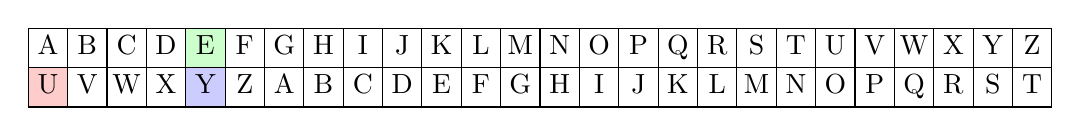
\begin{tikzpicture}
   \foreach \i in {0,...,3} {
      \node[draw, minimum size = 0.5cm, inner sep = 0pt]
      at (\i*0.5,0) {\strut\symbol{\numexpr`A+\i\relax}};
   }
   \foreach \i in {4,...,4} {
      \node[draw, minimum size = 0.5cm, inner sep = 0pt, fill = green!20]
      at (\i*0.5,0) {\strut\symbol{\numexpr`A+\i\relax}};
   }
   \foreach \i in {5,...,25} {
      \node[draw, minimum size = 0.5cm, inner sep = 0pt]
      at (\i*0.5,0) {\strut\symbol{\numexpr`A+\i\relax}};
   }

   \foreach \i in {0,...,0} {
      \foreach \j in {20,...,20} {
         \edef\k{\ifnum\numexpr\i+\j\relax>25
            \the\numexpr\i+\j-26\relax
            \else
            \the\numexpr\i+\j\relax
         \fi}
         \node[draw, minimum size = 0.5cm, inner sep = 0pt, fill = red!20]
         at (\i*0.5,-0.5) {\strut\symbol{\numexpr`A+\k\relax}};
      }
   }
   \foreach \i in {1,...,3} {
      \foreach \j in {20,...,20} {
         \edef\k{\ifnum\numexpr\i+\j\relax>25
            \the\numexpr\i+\j-26\relax
            \else
            \the\numexpr\i+\j\relax
         \fi}
         \node[draw, minimum size = 0.5cm, inner sep = 0pt]
         at (\i*0.5,-0.5) {\strut\symbol{\numexpr`A+\k\relax}};
      }
   }
   \foreach \i in {4,...,4} {
      \foreach \j in {20,...,20} {
         \edef\k{\ifnum\numexpr\i+\j\relax>25
            \the\numexpr\i+\j-26\relax
            \else
            \the\numexpr\i+\j\relax
         \fi}
         \node[draw, minimum size = 0.5cm, inner sep = 0pt, fill = blue!20]
         at (\i*0.5,-0.5) {\strut\symbol{\numexpr`A+\k\relax}};
      }
   }
   \foreach \i in {5,...,25} {
      \foreach \j in {20,...,20} {
         \edef\k{\ifnum\numexpr\i+\j\relax>25
            \the\numexpr\i+\j-26\relax
            \else
            \the\numexpr\i+\j\relax
         \fi}
         \node[draw, minimum size = 0.5cm, inner sep = 0pt]
         at (\i*0.5,-0.5) {\strut\symbol{\numexpr`A+\k\relax}};
      }
   }
\end{tikzpicture}

\vspace{0.5cm}

% Ligne 5
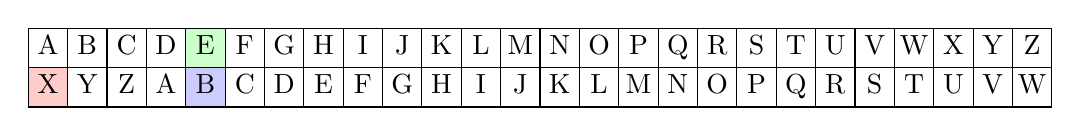
\begin{tikzpicture}
   \foreach \i in {0,...,3} {
      \node[draw, minimum size = 0.5cm, inner sep = 0pt]
      at (\i*0.5,0) {\strut\symbol{\numexpr`A+\i\relax}};
   }
   \foreach \i in {4,...,4} {
      \node[draw, minimum size = 0.5cm, inner sep = 0pt, fill = green!20]
      at (\i*0.5,0) {\strut\symbol{\numexpr`A+\i\relax}};
   }
   \foreach \i in {5,...,25} {
      \node[draw, minimum size = 0.5cm, inner sep = 0pt]
      at (\i*0.5,0) {\strut\symbol{\numexpr`A+\i\relax}};
   }

   \foreach \i in {0,...,0} {
      \foreach \j in {23,...,23} {
         \edef\k{\ifnum\numexpr\i+\j\relax>25
            \the\numexpr\i+\j-26\relax
            \else
            \the\numexpr\i+\j\relax
         \fi}
         \node[draw, minimum size = 0.5cm, inner sep = 0pt, fill = red!20]
         at (\i*0.5,-0.5) {\strut\symbol{\numexpr`A+\k\relax}};
      }
   }
   \foreach \i in {1,...,3} {
      \foreach \j in {23,...,23} {
         \edef\k{\ifnum\numexpr\i+\j\relax>25
            \the\numexpr\i+\j-26\relax
            \else
            \the\numexpr\i+\j\relax
         \fi}
         \node[draw, minimum size = 0.5cm, inner sep = 0pt]
         at (\i*0.5,-0.5) {\strut\symbol{\numexpr`A+\k\relax}};
      }
   }
   \foreach \i in {4,...,4} {
      \foreach \j in {23,...,23} {
         \edef\k{\ifnum\numexpr\i+\j\relax>25
            \the\numexpr\i+\j-26\relax
            \else
            \the\numexpr\i+\j\relax
         \fi}
         \node[draw, minimum size = 0.5cm, inner sep = 0pt, fill = blue!20]
         at (\i*0.5,-0.5) {\strut\symbol{\numexpr`A+\k\relax}};
      }
   }
   \foreach \i in {5,...,25} {
      \foreach \j in {23,...,23} {
         \edef\k{\ifnum\numexpr\i+\j\relax>25
            \the\numexpr\i+\j-26\relax
            \else
            \the\numexpr\i+\j\relax
         \fi}
         \node[draw, minimum size = 0.5cm, inner sep = 0pt]
         at (\i*0.5,-0.5) {\strut\symbol{\numexpr`A+\k\relax}};
      }
   }
\end{tikzpicture}

\vspace{1cm}


\begin{tikzpicture}
   \node [anchor = center] (first) {L};
   \node [anchor = center, right = 0cm of first] (second) {I};
   \node [anchor = center, right = 0cm of second] (third) {N};
   \node [anchor = center, right = 0cm of third] (fourth) {U};
   \node [anchor = center, right = 0cm of fourth] (fifth) {X};
\end{tikzpicture}

\end{document}
